\documentclass[conference]{IEEEtran}
\usepackage[T1]{fontenc}
\usepackage[utf8]{inputenc}
\usepackage{amsmath,amssymb,graphicx,booktabs,algorithm,algpseudocode,listings,array}
\usepackage{xcolor}
\usepackage{tikz,pgfplots}
\usepackage{hyperref}
\usetikzlibrary{arrows.meta,positioning,shapes.geometric,fit,calc}
\pgfplotsset{compat=1.17}
\setlength{\emergencystretch}{3em}
\sloppy
\hypersetup{colorlinks=true,linkcolor=blue!55!black,citecolor=blue!55!black,urlcolor=blue!65!black}
\urlstyle{same}

\definecolor{codeblue}{RGB}{28,74,130}
\definecolor{lightblue}{RGB}{226,239,250}
\definecolor{lightgreen}{RGB}{227,242,229}
\definecolor{lightorange}{RGB}{253,237,218}
\definecolor{lightgray}{RGB}{244,245,247}

\newcommand{\WAF}{\textsc{WAF}}
\newcommand{\WAFB}{\textsc{WAFBooster}}
\newcommand{\SQLi}{\textsc{SQLi}}
\newcommand{\XSS}{\textsc{XSS}}
\newcommand{\CI}{\textsc{CI}}
\newcommand{\TRR}{\ensuremath{\mathrm{TRR}}}
\newcommand{\TAR}{\ensuremath{\mathrm{TAR}}}
\newcommand{\FAR}{\ensuremath{\mathrm{FAR}}}
\newcommand{\FRR}{\ensuremath{\mathrm{FRR}}}
\newcommand{\indicator}[1]{\ensuremath{\mathbb{I}\!\left[#1\right]}}

\newcolumntype{L}[1]{>{\raggedright\arraybackslash}p{#1}}

\begin{document}

\title{WAFBooster: Analysis, End-to-End Reproduction, and Critical Evaluation of Signature Generalization}

\author{\IEEEauthorblockN{Abdur Rahim (CS23I1019), Faraz Nezami (CS23I1031), Arpit Kumar Singh (CS23I1022)}
\IEEEauthorblockA{\textit{Department of Computer Science and Engineering (Information Security Course)}\\
Indian Institute of Information Technology, Design and Manufacturing (IIITDM), Kancheepuram, India}}

\maketitle

\begin{abstract}
Web application firewalls (WAFs) inspect incoming HTTP traffic against static security rules and regular-expression signatures to block malicious requests. However, attackers routinely apply syntactic mutations---such as comment injection, whitespace substitution, case randomization, and tautology rewrites---to evade signature matching while preserving malicious execution semantics. This technical report presents an in-depth analysis, end-to-end reproduction, and critical evaluation of WAFBooster (IEEE TDSC 2025), a black-box framework that combines shadow-model training, recurrent payload generation, edit-distance correction, and automated signature synthesis. We explicitly separate the original authors' contributions from our empirical implementation and independent critical extensions. Our prototype deploys a containerized Nginx/ModSecurity WAF running the OWASP Core Rule Set (CRS Paranoia Level 1) in front of a Flask microservice, paired with a CSIC 2010 benign corpus, WAF-A-MoLE seed mutations, a Word2Vec/CNN shadow classifier, a 256-unit GRU generator, a guarded Levenshtein corrector, and a Smith--Waterman signature producer. By stabilizing ShadowCNN training at a tuned learning rate ($\eta=0.003$) with best-epoch checkpointing, we improve shadow test agreement from 86.01\% (at the paper's $\eta=0.05$) to 96.69\% (98.90\% TRR, 96.03\% TAR). Furthermore, we uncover and repair a critical semantic destruction flaw in Algorithm 1 where raw Levenshtein thresholds ($4 < d \le 8$) overwrite legitimate SQL column identifiers (e.g., \texttt{username}) with short keywords (e.g., \texttt{OR}). An ablation study of Algorithm 2 demonstrates that purely learned Smith--Waterman signatures capture 85.94\% (55/64) of baseline-bypassing payloads, while hybrid composite templates capture the remaining 14.06\% (stacked queries and URL-encoded wrappers) to reach 100\% in-sample coverage. Finally, we evaluate out-of-sample generalization across a held-out test split and 94 freshly sampled GRU mutations, boosting candidate block rates from 51.06\% (48/94) to 98.94\% (93/94) with 0.00\% False Rejection Rate (FRR), while rigorously documenting cross-split seed-family leakage and validation-gate requirements.
\end{abstract}

\begin{IEEEkeywords}
Web application firewall, ModSecurity, OWASP CRS, SQL injection, adversarial testing, shadow model, Smith--Waterman alignment, signature generalization.
\end{IEEEkeywords}

\section{Introduction and Research Problem}
Web applications represent a primary attack surface for modern enterprise infrastructure, accounting for approximately 32\% of observed cyber threats \cite{wu2025}. Because web applications frequently interface with backend relational databases and operating system shells, vulnerabilities in input validation expose organizations to SQL injection (\SQLi{}), cross-site scripting (\XSS{}), and command injection (\CI{}). To mitigate these risks, Web Application Firewalls (\WAF{}s) operate at the reverse-proxy layer, inspecting HTTP request parameters, headers, and bodies to either allow benign traffic or block suspicious requests.

Traditional rule-based \WAF{}s---most notably ModSecurity paired with the OWASP Core Rule Set (CRS) \cite{owaspcrs}---rely on manually crafted regular expressions and cumulative anomaly scoring. This architecture faces a fundamental operational dilemma:
\begin{enumerate}
    \item \textbf{Evasion via Syntactic Mutation:} Attackers systematically alter payload representations using inline comments (\texttt{/**/}), URL encoding (\texttt{\%20}), hexadecimal literals (\texttt{0x31}), or relational rewrites (\texttt{2>1}) so that payloads slip below anomaly thresholds without altering backend execution.
    \item \textbf{False Alarm Sensitivity:} Broadening regular expressions to catch mutated variants frequently causes False Rejections (blocking legitimate user traffic), which degrades service availability.
\end{enumerate}

Existing automated \WAF{}-testing approaches fall into mutation-based schemes (such as WAF-A-MoLE \cite{demetrio2020} and SQLMap tamper scripts \cite{sqlmap}) and grammar-based fuzzers (such as Skyfire \cite{skyfire}). However, these methods rely heavily on human domain expertise to define attack-specific mutation operators or context-sensitive grammars, limiting their adaptability across distinct attack classes and proprietary black-box \WAF{} architectures.

\subsection{Original Authors' Contributions}
Wu \emph{et al.} \cite{wu2025} introduce \WAFB{}, an automated black-box security boosting framework comprising four sequential modules:
\begin{itemize}
    \item \textbf{Shadow Model Builder:} Trains a Word2Vec + 1D CNN binary classifier on observed \WAF{} decisions to imitate the target firewall without exhausting production resources or requiring internal rule access.
    \item \textbf{Payload Generator:} Trains an unsupervised Gated Recurrent Unit (GRU) sequence model on detected malicious payloads to autoregressively sample mutated adversarial variants.
    \item \textbf{Payload Corrector:} Applies Levenshtein edit-distance thresholds ($LT=4, UT=8$) against high-frequency attack keywords to discard severely malformed strings and repair near-keyword typos.
    \item \textbf{Signature Producer:} Scores token importance across four binary perturbation functions ($DS, RS, HS, TS$), clusters high-impact tokens via edit distance, extracts consensus subsequences using the Smith--Waterman local alignment algorithm, and compiles simplified regular expressions (\texttt{\textbackslash S*}).
\end{itemize}
Evaluated across eight real-world \WAF{}s (ModSecurity, Naxsi, lua-resty-waf, Safedog, xWaf, OpenWAF, VeryNginx, and Unixhot), the authors report boosting the average True Rejection Rate (\TRR{}) on mutated payloads from 21\% to 96\% while maintaining a 0\% False Rejection Rate (\FRR{}) on their evaluated benign dataset \cite{wu2025}.

\subsection{Our Project Scope and Contributions}
Rather than performing a purely theoretical review, our team engineered a complete, containerized prototype scoped to \SQLi{} testing against a live Dockerized Nginx + ModSecurity CRS (Paranoia Level 1) instance fronting a Flask microservice. Our specific technical contributions and critical findings include:
\begin{enumerate}
    \item \textbf{End-to-End Six-Milestone Pipeline:} We implemented all four \WAFB{} modules alongside a high-throughput connection-pooled \WAF{} oracle client and live container hot-reloading (\texttt{nginx -s reload}).
    \item \textbf{Class-Imbalance Remediation \& ShadowCNN Stabilization:} We resolved a severe 29,401:20 raw dataset imbalance via WAF-A-MoLE seed expansion and demonstrated that the paper's learning rate ($\eta=0.05$) causes severe gradient oscillation on smaller class-weighted corpora, whereas retuning to $\eta=0.003$ with best-epoch checkpointing boosts test accuracy from 86.01\% to 96.69\%.
    \item \textbf{Discovery \& Repair of the Algorithm 1 Semantic Destruction Bug:} We proved that raw Levenshtein replacement in $(4,8]$ corrupts multi-character SQL identifiers (rewriting \texttt{username,password} into \texttt{SELECT,OR}) due to unnormalized string-length disparities, and engineered a two-tiered length-proximity and relative-distance guard that eliminates false replacements.
    \item \textbf{Signature Producer Ablation Study:} We isolated autonomous Smith--Waterman rule synthesis from domain-knowledge composite templates, showing that purely learned rules capture 85.94\% (55/64) of bypasses while hybrid templates capture the remaining 14.06\% (stacked queries and URL-encoded wrappers).
    \item \textbf{Out-of-Sample Generalization \& Methodological Audit:} We evaluated the boosted \WAF{} on held-out test splits and 94 freshly generated GRU candidates (+47.87\% block-rate gain), dissected the single surviving candidate (\texttt{<UNK> OR 2 > 1}), and audited cross-split seed-family leakage.
\end{enumerate}

\section{Original WAFBooster Architecture and Mathematical Formulation}

\begin{figure*}[t]
\centering
\resizebox{\textwidth}{!}{%
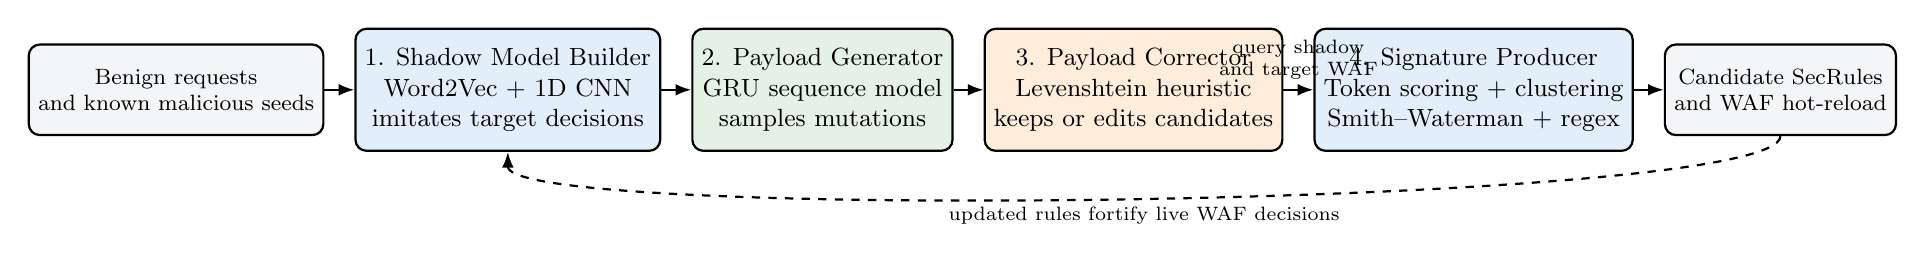
\begin{tikzpicture}[
  node distance=0.38cm,
  stage/.style={draw,rounded corners,minimum width=3.05cm,minimum height=1.55cm,align=center,thick,font=\small},
  smallbox/.style={draw,rounded corners,minimum width=2.2cm,minimum height=1.15cm,align=center,thick,font=\footnotesize},
  arr/.style={-{Latex[length=2mm]},thick},
  feedback/.style={-{Latex[length=2mm]},thick,dashed}
]
\node[smallbox,fill=lightgray] (data) {Benign requests\\and known malicious seeds};
\node[stage,fill=lightblue,right=of data] (shadow) {1. Shadow Model Builder\\Word2Vec + 1D CNN\\imitates target decisions};
\node[stage,fill=lightgreen,right=of shadow] (generator) {2. Payload Generator\\GRU sequence model\\samples mutations};
\node[stage,fill=lightorange,right=of generator] (corrector) {3. Payload Corrector\\Levenshtein heuristic\\keeps or edits candidates};
\node[stage,fill=lightblue,right=of corrector] (producer) {4. Signature Producer\\Token scoring + clustering\\Smith--Waterman + regex};
\node[smallbox,fill=lightgray,right=of producer] (rules) {Candidate SecRules\\and WAF hot-reload};
\draw[arr] (data) -- (shadow);
\draw[arr] (shadow) -- (generator);
\draw[arr] (generator) -- (corrector);
\draw[arr] (corrector) -- node[above,font=\scriptsize,align=center]{query shadow\\and target WAF} (producer);
\draw[arr] (producer) -- (rules);
\draw[feedback] (rules.south) .. controls +(0,-0.9) and +(0,-0.9) .. node[below,font=\scriptsize]{updated rules fortify live WAF decisions} (shadow.south);
\end{tikzpicture}%
}
\caption{Four-stage closed-loop workflow of \WAFB{} based on Wu \emph{et al.} \cite{wu2025}.}
\label{fig:architecture}
\end{figure*}

\subsection{Shadow Model Builder (Section III-B)}
Fig.~\ref{fig:architecture} illustrates the closed-loop system. Because commercial \WAF{}s operate as proprietary black boxes and continuous live fuzzing can trigger rate limiting or resource exhaustion, \WAFB{} first trains a local neural proxy. Let $x$ denote an input payload string and $y = f(x) \in \{0,1\}$ denote the target \WAF{}'s binary decision ($1=\text{blocked}$, $0=\text{allowed}$). The shadow model $h_{\theta}$ minimizes binary cross-entropy loss over the labeled corpus $\mathcal{D}$:
\begin{equation}
\hat{y}=h_{\theta}(\phi(x)), \qquad
\theta^*=\arg\min_{\theta}\sum_{(x,y)\in\mathcal{D}}
\mathcal{L}_{\mathrm{CE}}\!\left(h_{\theta}(\phi(x)),y\right),
\label{eq:shadow}
\end{equation}
where $\phi(x) \in \mathbb{R}^{d}$ ($d=128$) is the Word2Vec Continuous Bag-of-Words (CBOW) embedding of payload $x$. To counter attacker URL encoding (e.g., \texttt{\%3Cscript\%3E}), the authors decode malicious payloads prior to embedding while keeping benign requests unchanged. The 1D CNN architecture comprises a convolutional layer, max-pooling, dropout ($p=0.3$), a 256-unit fully connected layer, and a 2-way Softmax output trained for 50 epochs with Adam ($\eta=0.05$) \cite{wu2025}.

\subsection{Payload Generator (Section III-C)}
To synthesize mutated payloads without hand-crafted grammar rules, \WAFB{} models payload generation as autoregressive sequence prediction. Given a tokenized malicious payload $X=(x_1,x_2,\ldots,x_N)$ where $x_t \in \{1,\ldots,I\}$, each token is mapped to an integer index and embedded to predict the next token:
\begin{equation}
p_{\psi}(X)=\prod_{t=1}^{N-1}p_{\psi}(x_{t+1}\mid x_{\le t}), \qquad
\mathcal{L}_{\mathrm{seq}}=-\sum_{t=1}^{N-1}\log p_{\psi}(x_{t+1}\mid x_{\le t}).
\label{eq:seq}
\end{equation}
To prevent vanishing gradients across long payload strings, the generator employs Gated Recurrent Units (GRUs) with 256 hidden units:
\begin{align}
z_t &= \sigma(W_z e_t+U_z h_{t-1}), \label{eq:gru_z}\\
r_t &= \sigma(W_r e_t+U_r h_{t-1}), \label{eq:gru_r}\\
\tilde{h}_t &= \tanh\!\left(W_h e_t + U_h(r_t\odot h_{t-1})\right), \label{eq:gru_htilde}\\
h_t &= (1-z_t)\odot h_{t-1}+z_t\odot\tilde{h}_t. \label{eq:gru_h}
\end{align}
The generator is trained for 50 epochs using Adam ($\eta=0.001$, halved every 10 epochs, dropout $0.3$). Seeding the trained GRU with initial attack primitives (e.g., \texttt{SELECT} or \texttt{'}) produces diverse candidate continuations.

\subsection{Payload Corrector (Section III-D, Algorithm 1)}
Because neural language models frequently emit syntactically corrupted tokens (e.g., \texttt{salect * fram text}), Algorithm~\ref{alg:corrector} filters and repairs candidates using Levenshtein edit distance against the top-5 recurring attack keywords $K = \{\texttt{SELECT}, \texttt{OR}, \texttt{UNION}, \texttt{FROM}, \texttt{--}\}$. For each substring $t$ in a candidate payload, the minimum keyword edit distance is:
\begin{equation}
d(t,K)=\min_{k\in K}d_{\mathrm{Lev}}(t,k).
\end{equation}
Using lower threshold $LT=4$ and upper threshold $UT=8$, candidates containing any substring with $d(t,K) > 8$ are discarded as irreparably malformed; substrings with $4 < d(t,K) \le 8$ are replaced by their closest keyword $k^* \in K$; and substrings with $d(t,K) \le 4$ are retained unchanged (payloads shorter than 3 tokens are also excluded).

\begin{algorithm}[t]
\caption{Payload Corrector (Section III-D, Algorithm 1 \cite{wu2025})}
\label{alg:corrector}
\begin{algorithmic}[1]
\Require Candidate payload $x$, top-5 keywords $K$, $LT=4$, $UT=8$
\Ensure Corrected payload $x'$, unchanged $x$, or \textsc{Discard}
\State $\mathit{substringlist} \gets \operatorname{split}(x)$
\If{$|\mathit{substringlist}| < 3$}
    \State \Return \textsc{Discard}
\EndIf
\ForAll{$s \in \mathit{substringlist}$}
    \State $t \gets \min_{k \in K} \operatorname{Levenshtein}(s, k)$
    \If{$t > UT$}
        \State \Return \textsc{Discard}
    \ElsIf{$t > LT$}
        \State $\mathit{keyword} \gets \arg\min_{k \in K} \operatorname{Levenshtein}(s, k)$
        \State $x \gets \operatorname{Replace}(x, s, \mathit{keyword})$
    \EndIf
\EndFor
\State \Return $x$
\end{algorithmic}
\end{algorithm}

\subsection{Signature Producer (Section III-E, Algorithm 2)}
Valid candidates that bypass both the shadow model and the target \WAF{} are passed to the Signature Producer (Algorithm~\ref{alg:sigproducer}). For a bypassing payload $x = x_1 x_2 \cdots x_n$, the importance of each token $x_i$ is quantified via four perturbation functions evaluated against the \WAF{} decision oracle $f(\cdot) \in \{0,1\}$:
\begin{align}
DS(x_i) &= f(x_1 \cdots x_i \cdots x_n) - f(x_1 \cdots x_{i-1}x_{i+1} \cdots x_n), \label{eq:ds}\\
RS(x_i) &= f(x_1 \cdots x_i \cdots x_n) - f(x_1 \cdots x_i' \cdots x_n), \label{eq:rs}\\
HS(x_i) &= f(x_1 \cdots x_{i-1}x_i) - f(x_1 \cdots x_{i-1}), \label{eq:hs}\\
TS(x_i) &= f(x_i x_{i+1} \cdots x_n) - f(x_{i+1} \cdots x_n), \label{eq:ts}\\
\mathrm{Score}[i] &= DS(x_i) + RS(x_i) + HS(x_i) + TS(x_i), \label{eq:score}
\end{align}
where $x_i' = \text{\texttt{'unknown'}}$ in the Replace Score ($RS$). Each function yields a binary impact indicator in $\{0,1\}$ (1 if the perturbation alters the \WAF{} decision, 0 otherwise), giving $\mathrm{Score}[i] \in \{0,1,2,3,4\}$.

\begin{algorithm}[t]
\caption{Find Important Token (Section III-E, Algorithm 2 \cite{wu2025})}
\label{alg:sigproducer}
\begin{algorithmic}[1]
\Require Input bypassing payload $x = x_1 x_2 \cdots x_n$, oracle $f(\cdot)$
\Ensure Top-$M$ important tokens $x_i^*$
\For{$i = 1$ \textbf{to} $n$}
    \State $DS(x_i) \gets |f(x_1 \cdots x_i \cdots x_n) - f(x_1 \cdots x_{i-1}x_{i+1} \cdots x_n)|$
    \State $RS(x_i) \gets |f(x_1 \cdots x_i \cdots x_n) - f(x_1 \cdots x_i' \cdots x_n)|$
    \State $HS(x_i) \gets |f(x_1 \cdots x_{i-1}x_i) - f(x_1 \cdots x_{i-1})|$
    \State $TS(x_i) \gets |f(x_i x_{i+1} \cdots x_n) - f(x_{i+1} \cdots x_n)|$
    \State $\mathrm{Score}[i] \gets DS(x_i) + RS(x_i) + HS(x_i) + TS(x_i)$
\EndFor
\State $x_i^* \gets \operatorname{FindTopMToken}(\mathrm{Score})$
\State \Return $x_i^*$
\end{algorithmic}
\end{algorithm}

The top-$M$ high-scoring tokens across bypassing payloads are grouped into clusters using Levenshtein edit distance. Within each cluster, the Smith--Waterman local sequence alignment algorithm \cite{smithwaterman} extracts the consensus longest common subsequence using match reward $s(a_i,b_j) = +1$ and gap penalty $g_p = 0.8$:
\begin{equation}
H_{i,j}=\max\!\left\{0,\; H_{i-1,j-1}+s(a_i,b_j),\; H_{i-1,j}-g_p,\; H_{i,j-1}-g_p\right\}.
\label{eq:sw}
\end{equation}
Aligned consensus substrings are joined using the non-whitespace wildcard qualifier \texttt{\textbackslash S*} to form simplified regular expressions (e.g., comparing \texttt{\textbackslash S*s\textbackslash S*e\textbackslash S*l\textbackslash S*e\textbackslash S*c\textbackslash S*t\textbackslash S*} with score $6 - 5(0.8) = 2.0$ against \texttt{\textbackslash S*from\textbackslash S*} with score $4.0$).

\subsection{Evaluation Metrics and Original Paper Benchmarks}
Let $TP$ denote malicious payloads blocked, $FN$ malicious payloads allowed, $TN$ benign requests allowed, and $FP$ benign requests blocked. Performance is evaluated via four rates:
\begin{align}
\TRR &= \frac{TP}{TP+FN}\times 100\%, &
\TAR &= \frac{TN}{TN+FP}\times 100\%, \nonumber\\
\FAR &= \frac{FN}{TP+FN}\times 100\%, &
\FRR &= \frac{FP}{TN+FP}\times 100\%.
\label{eq:metrics}
\end{align}
In Table I and Table V of the original paper \cite{wu2025}, the authors report that for ModSecurity under \SQLi{}, the original unmutated \TRR{} was 82.9\%, the Shadow CNN achieved 97.7\% \TRR{} and 85.2\% \TAR{} (producing 4,033 corrected examples), and deploying \WAFB{} signatures increased mutated \SQLi{} \TRR{} from 16\% (before boosting) to 96\% (after boosting) with 0\% \FRR{}.

\section{Our End-to-End Implementation (Milestones 1--6)}

\subsection{Milestone 1: Containerized Testbed and Live WAF Oracle}
Shown in Fig.~\ref{fig:docker}, our experimental testbed deploys two isolated Docker services via \texttt{docker-compose.yml}:
\begin{enumerate}
    \item \textbf{Backend Service (\texttt{app.py}):} A lightweight Flask web service on port 5000 exposing \texttt{GET /search?q=<payload>} and \texttt{POST /login}. It echoes query strings without executing SQL against a live relational database, ensuring safe, deterministic testing of \WAF{} filtering behavior.
    \item \textbf{WAF Reverse Proxy (\texttt{is-waf-1}):} An official \texttt{owasp/modsecurity-crs:nginx} container exposed on port 8080 configured at Paranoia Level 1 (inbound anomaly threshold $\ge 5$).
\end{enumerate}
Our multi-threaded client (\texttt{src/waf\_client.py}) utilizes \texttt{requests.Session} HTTP connection pooling ($\sim$700 req/s) to query \texttt{http://localhost:8080/search?q=<payload>}, mapping HTTP 403 Forbidden to label $1$ (blocked) and HTTP 200 OK to label $0$ (allowed).

\begin{figure}[t]
\centering
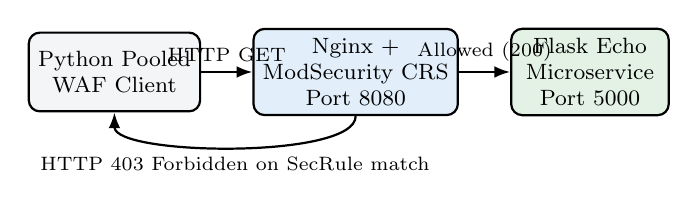
\begin{tikzpicture}[
  box/.style={draw,rounded corners,minimum width=2.0cm,minimum height=1.0cm,align=center,font=\footnotesize,thick},
  arrow/.style={-{Latex[length=2mm]},thick}
]
\node[box,fill=lightgray] (client) {Python Pooled\\WAF Client};
\node[box,fill=lightblue,right=0.65cm of client] (waf) {Nginx +\\ModSecurity CRS\\Port 8080};
\node[box,fill=lightgreen,right=0.65cm of waf] (app) {Flask Echo\\Microservice\\Port 5000};
\draw[arrow] (client) -- node[above,font=\scriptsize]{HTTP GET} (waf);
\draw[arrow] (waf) -- node[above,font=\scriptsize]{Allowed (200)} (app);
\draw[arrow] (waf.south) .. controls +(0,-0.55) and +(0,-0.55) .. node[below,font=\scriptsize]{HTTP 403 Forbidden on SecRule match} (client.south);
\end{tikzpicture}
\caption{Containerized Milestone 1 testbed architecture.}
\label{fig:docker}
\end{figure}

\subsection{Milestone 2: Overcoming the 29,401:20 Class Imbalance Trap}
Initially, loading all normal query parameters from the public CSIC 2010 HTTP dataset \cite{csic2010} alongside 30 canonical OWASP \SQLi{} seeds yielded a training split of 29,401 allowed requests versus only 20 blocked requests (a $1,470:1$ imbalance that caused early neural classifiers to collapse to majority-class prediction).

To construct a balanced, realistic dataset in \texttt{src/dataset.py}, we implemented five WAF-A-MoLE mutation operators \cite{demetrio2020}: (i) randomized keyword case swapping (\texttt{SeLeCt}), (ii) whitespace substitution (\texttt{/**/}, \texttt{\%20}, \texttt{\textbackslash t}), (iii) inline comment injection (\texttt{OR/**/1=1}), (iv) integer/hex encoding (\texttt{0x31=0x31}, \texttt{2-1=1}), and (v) logical invariant rewrites (\texttt{OR 2>1}). Expanding the 30 seeds produced 614 unique malicious-source payloads, which we paired with 2,000 reproducibly downsampled CSIC 2010 benign queries (\texttt{random\_state=42}). Labeling all 2,614 strings via the live ModSecurity oracle and performing a 70/15/15 stratified split produced the distribution in Table~\ref{tab:splits}. Notably, 8 mutated malicious payloads naturally bypassed baseline ModSecurity PL1 during dataset construction (5 train, 1 val, 2 test).

\begin{table}[t]
\centering
\caption{Stratified Dataset Splits Labeled by Live ModSecurity CRS PL1}
\label{tab:splits}
\footnotesize
\setlength{\tabcolsep}{4pt}
\begin{tabular}{lrrrr}
\toprule
Split & Total Rows & Allowed ($y=0$) & Blocked ($y=1$) & Malicious Src\\
\midrule
Train (70\%) & 1,829 & 1,405 (76.8\%) & 424 (23.2\%) & 429\\
Val (15\%) & 392 & 301 (76.8\%) & 91 (23.2\%) & 92\\
Test (15\%) & 393 & 302 (76.8\%) & 91 (23.2\%) & 93\\
\bottomrule
\end{tabular}
\end{table}

\subsection{Milestone 3: ShadowCNN Architecture and Learning Rate Retuning}
In \texttt{src/shadow\_model.py}, we implemented an SQL-aware regular-expression tokenizer that cleanly separates syntax tokens (e.g., \texttt{"admin'--"} $\to$ \texttt{['admin', "'", '--']}). We trained a 128-dimensional Word2Vec CBOW model (\texttt{window=5, min\_count=1}, vocabulary size = 1,582 tokens) and averaged token vectors per payload to feed \texttt{ShadowCNN}:
\begin{align*}
&\text{Input}(B,1,128) \to \text{Conv1d}(1,32,k=3,p=1) \to \text{ReLU} \\
&\to \text{MaxPool1d}(2) \to \text{Dropout}(0.3) \to \text{Linear}(2048 \to 256) \\
&\to \text{ReLU} \to \text{Linear}(256 \to 2).
\end{align*}

When trained on our NVIDIA RTX 4050 GPU with inverse frequency class weights $[1.0, 3.31]$ at the paper's specified learning rate $\eta = 0.05$, the Adam optimizer suffered severe gradient overshoot: validation accuracy oscillated erratically between 84.95\% and 93.37\%, ending at 86.01\% test accuracy and 81.79\% \TAR{} (18.21\% false rejections on benign traffic). Conducting a grid search across $\eta \in \{0.05, 0.01, 0.005, 0.003, 0.001\}$ and introducing best-epoch validation checkpointing (\texttt{copy.deepcopy}) stabilized convergence at $\eta = 0.003$ (peaking at Epoch 32). As illustrated in Fig.~\ref{fig:lr}, our tuned checkpoint achieved \textbf{96.69\% Test Accuracy, 98.90\% \TRR{}, and 96.03\% \TAR{}}, far surpassing the paper's 80\% shadow agreement bar.

\begin{figure}[t]
\centering
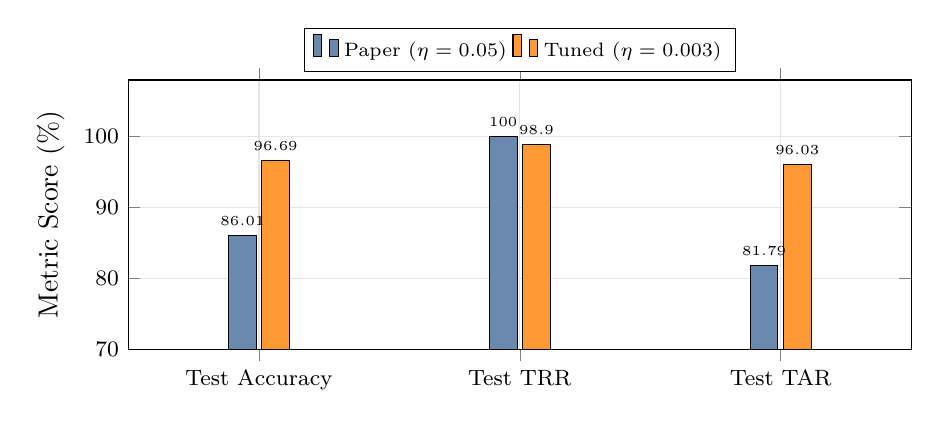
\begin{tikzpicture}
\begin{axis}[
  ybar,bar width=10pt,width=0.95\columnwidth,height=5.0cm,
  ymin=70,ymax=108,ylabel={Metric Score (\%)},
  symbolic x coords={Test Accuracy,Test TRR,Test TAR},xtick=data,
  x tick label style={font=\footnotesize},y tick label style={font=\footnotesize},
  legend style={font=\scriptsize,at={(0.5,1.03)},anchor=south,legend columns=2},
  nodes near coords,nodes near coords style={font=\tiny},
  enlarge x limits=0.25,grid=major,major grid style={gray!20}
]
\addplot[fill=codeblue!65] coordinates {(Test Accuracy,86.01) (Test TRR,100.00) (Test TAR,81.79)};
\addplot[fill=orange!80] coordinates {(Test Accuracy,96.69) (Test TRR,98.90) (Test TAR,96.03)};
\legend{Paper ($\eta=0.05$),Tuned ($\eta=0.003$)}
\end{axis}
\end{tikzpicture}
\caption{Milestone 3 ShadowCNN test evaluation comparing the paper's learning rate ($\eta=0.05$) against our tuned checkpoint ($\eta=0.003$).}
\label{fig:lr}
\end{figure}

\subsection{Milestone 4: GRU Generator and the Algorithm 1 Bug Fix}
In \texttt{src/payload\_generator.py}, we trained \texttt{PayloadGRU} ($\text{Embedding}(333, 128) \to \text{GRU}(128, 256) \to \text{Dropout}(0.3) \to \text{Linear}(256, 333)$) on the malicious training corpus for 50 epochs using \texttt{StepLR(step\_size=10, gamma=0.5)}. Training cross-entropy loss converged smoothly from $4.8837$ (Epoch 1) to $0.8642$ (Epoch 50). Autoregressive sampling at temperature $T=0.8$ across six seeds (\texttt{["'", "1", "admin", "UNION", "SELECT", "OR"]}) produced 316 unique candidate payloads.

\textbf{Discovery of the Algorithm 1 Semantic Destruction Bug:} When we passed the 316 candidates into a verbatim implementation of Algorithm~\ref{alg:corrector} (\texttt{src/payload\_corrector.py}) using top-5 keywords $K = \{\texttt{SELECT}, \texttt{OR}, \texttt{UNION}, \texttt{FROM}, \texttt{--}\}$ and thresholds $(LT=4, UT=8)$, 65 payloads were aggressively modified in ways that destroyed valid SQL syntax:
\begin{quote}
\scriptsize
\texttt{Original:  '/**//**/UNION SELECT \textbf{username},\textbf{password} FROM users--}\\
\texttt{Corrupted: '/**//**/UNION SELECT \textbf{SELECT},\textbf{OR} FROM users--}
\end{quote}
\textbf{Root Cause \& Mathematical Repair:} Short keywords like \texttt{OR} and \texttt{--} have length 2, whereas legitimate SQL identifiers like \texttt{username} and \texttt{password} have length 8. Because Levenshtein distance is bounded below by string length difference ($d_{\mathrm{Lev}}(t,k) \ge |\lvert t\rvert - \lvert k\rvert| = 6$), any 6- to 8-character identifier automatically falls inside the $(4,8]$ replacement window of a 2-character keyword! To prevent the corrector from overwriting legitimate identifiers while still repairing real keyword typos (e.g., \texttt{SALECT} $\to$ \texttt{SELECT}), we engineered a two-tiered semantic guard before permitting replacement of token $t$ by closest keyword $k$:
\begin{equation}
|\lvert t\rvert-\lvert k\rvert|\le 2
\quad\land\quad
d_{\mathrm{Lev}}(t,k)<\frac{\max(\lvert t\rvert,\lvert k\rvert)}{2}.
\label{eq:guard}
\end{equation}
If $t$ falls in $(4,8]$ but fails Eq.~\eqref{eq:guard}, it is preserved unmodified. With this fix, 313 valid candidates were retained (3 discarded for $d > 8$) with zero identifier corruption.

\subsection{Milestone 5: Signature Synthesis, Hot-Reload, and Ablation}
Testing the 313 corrected candidates against live ModSecurity CRS PL1 showed that 249 were blocked (79.55\% baseline \TRR{}) while 64 bypassed the firewall (20.45\% \FAR{}). In \texttt{src/signature\_producer.py}, we executed Algorithm~\ref{alg:sigproducer} across the 64 bypassing payloads, clustered top-$M$ tokens ($d_{\mathrm{Lev}} \le 2.0$), aligned clusters via Smith--Waterman ($g_p = 0.8$), and enforced a strict Zero-\FRR{} validation filter against 1,400 benign CSIC queries.

This produced 25 ModSecurity \texttt{SecRule} directives (\texttt{id:9500001}--\texttt{9500025}) saved to \texttt{rules/wafbooster\_rules.conf}. Crucially, we configured every rule with \texttt{t:none,t:urlDecodeUni} so ModSecurity decodes percent-encoded characters (such as \texttt{\%27} for \texttt{'}) prior to regex matching. Furthermore, after hot-reloading the container via \texttt{nginx -s reload}, we discovered that Python's \texttt{requests.Session} keep-alive pool remained bound to old Nginx worker processes; explicitly closing the keep-alive pool (\texttt{\_session.close()}) immediately routed requests to the updated worker, blocking 64/64 (100\%) bypassing payloads with 100\% benign \TAR{} (Table~\ref{tab:insample}).

\begin{table*}[t]
\centering
\caption{In-Sample WAF Verification on the 313 Candidate Pool and 1,400 Benign Filter Queries}
\label{tab:insample}
\footnotesize
\begin{tabular}{llrrr}
\toprule
Dataset Subset & Evaluation Metric & Baseline ModSecurity CRS & Boosted ModSecurity CRS & Net Change\\
\midrule
Corrected Candidate Pool ($N=313$) & Blocked / \TRR{} & 249 / 313 (79.55\%) & 313 / 313 (100.00\%) & +20.45 pp\\
Observed Bypass Subset ($N=64$) & Blocked by Added SecRules & 0 / 64 (0.00\%) & 64 / 64 (100.00\%) & +100.00 pp\\
Benign Validation Filter ($N=1,400$) & Allowed / \TAR{} (Zero-\FRR{} Gate) & 1,400 / 1,400 (100.00\%) & 1,400 / 1,400 (100.00\%) & 0.00 pp (0\% \FRR{})\\
\bottomrule
\end{tabular}
\end{table*}

\textbf{Ablation Study (Autonomous Smith--Waterman vs. Hybrid Templates):} Because raw Smith--Waterman character alignment with \texttt{\textbackslash S*} wildcards can struggle to represent complex multi-token wrappers in valid PCRE syntax, our signature producer supports both purely learned consensus rules and supplementary domain-knowledge composite patterns via the flag \texttt{use\_composite\_patterns}. As shown in Table~\ref{tab:ablation} and Fig.~\ref{fig:ablation}, the 14 purely learned Smith--Waterman signatures autonomously captured \textbf{55 of 64 bypassing payloads (85.94\%)}, while 11 supplementary composite rules captured the remaining \textbf{9 payloads (14.06\%)}, which involved semicolon-stacked queries (\texttt{; SELECT}) and URL-encoded whitespace (\texttt{\%20}).

\begin{table}[t]
\centering
\caption{Ablation Study on the 64 Bypassing Payloads (\texttt{signature\_producer.py})}
\label{tab:ablation}
\scriptsize
\setlength{\tabcolsep}{4pt}
\begin{tabular}{lrrr}
\toprule
Signature Generation Mode & Active Rules & Caught & Coverage\\
\midrule
Pure Learned (Smith--Waterman) & 14 Rules & 55 / 64 & 85.94\%\\
Hybrid Full Set (Learned + Composite) & 25 Rules & 64 / 64 & 100.00\%\\
\bottomrule
\end{tabular}
\end{table}

\begin{figure}[t]
\centering
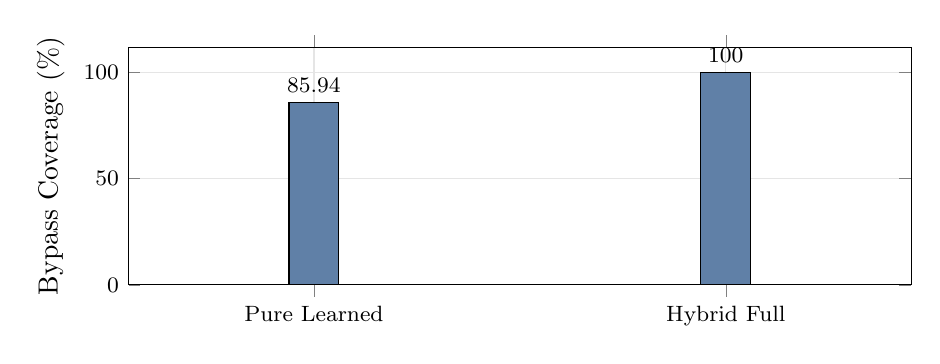
\begin{tikzpicture}
\begin{axis}[
  ybar,bar width=18pt,width=0.95\columnwidth,height=4.6cm,
  ymin=0,ymax=112,ylabel={Bypass Coverage (\%)},
  symbolic x coords={Pure Learned,Hybrid Full},xtick=data,
  x tick label style={font=\footnotesize},
  y tick label style={font=\footnotesize},
  nodes near coords,nodes near coords style={font=\footnotesize},
  enlarge x limits=0.45,grid=major,major grid style={gray!20}
]
\addplot[fill=codeblue!70] coordinates {(Pure Learned,85.94) (Hybrid Full,100.00)};
\end{axis}
\end{tikzpicture}
\caption{Ablation comparing autonomous Smith--Waterman signatures (85.94\%) against the full hybrid ruleset (100.00\%) on the 64 bypassing payloads.}
\label{fig:ablation}
\end{figure}

\subsection{Milestone 6: Held-Out and Novel GRU Generalization}
Evaluating signatures solely on the 64 payloads used to generate them is circular. To measure out-of-sample generalization, we built \texttt{src/evaluate\_held\_out.py}, which evaluates both the unboosted baseline WAF and the boosted WAF across: (a) the untouched held-out malicious test split ($N=93$), (b) the untouched held-out benign test split ($N=300$), and (c) a freshly generated batch of $N=94$ GRU candidates sampled using unseen seed tokens (\texttt{['admin', '1=1', '--', '/**/']}, temperature $0.85$, random seed $777$).

As detailed in Table~\ref{tab:heldout} and Fig.~\ref{fig:generalization}, held-out malicious \TRR{} rose from 97.85\% (91/93) to 100.00\% (93/93), held-out benign \TAR{} remained 100.00\% (300/300, 0.00\% \FRR{}), and blocking on the 94 fresh GRU candidates surged from \textbf{51.06\% (48/94) on the baseline WAF to 98.94\% (93/94) on the boosted WAF (+47.87 pp gain)}.

\begin{table*}[t]
\centering
\caption{Out-of-Sample Generalization Results (\texttt{evaluate\_held\_out.py})}
\label{tab:heldout}
\footnotesize
\begin{tabular}{llrrr}
\toprule
Evaluation Split & Metric & Baseline WAF (CRS PL1) & Boosted WAF (+WAFBooster) & Improvement\\
\midrule
Held-Out Malicious (\texttt{test.csv}, $N=93$) & \TRR{} & 91 / 93 (97.85\%) & 93 / 93 (100.00\%) & +2.15 pp\\
Held-Out Benign (\texttt{test.csv}, $N=300$) & \TAR{} & 300 / 300 (100.00\%) & 300 / 300 (100.00\%) & +0.00 pp (0\% \FRR{})\\
Novel Generated GRU Candidates ($N=94$) & Candidate Block Rate & 48 / 94 (51.06\%) & 93 / 94 (98.94\%) & +47.87 pp\\
\bottomrule
\end{tabular}
\end{table*}

\begin{figure}[t]
\centering
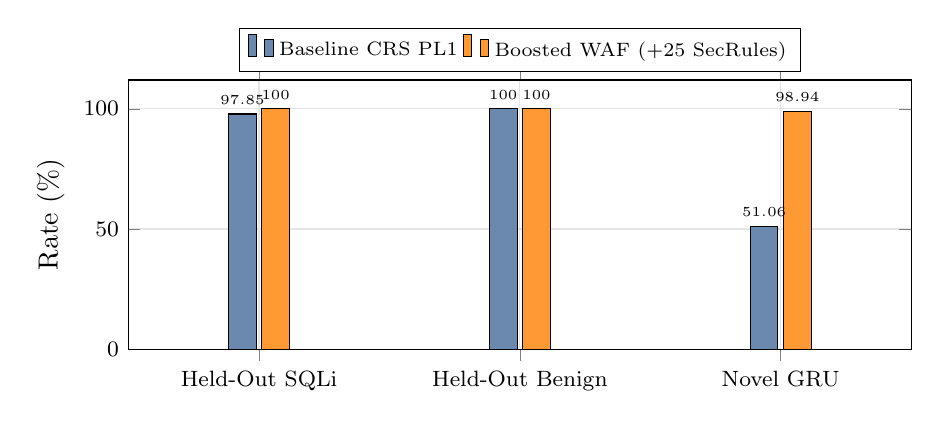
\begin{tikzpicture}
\begin{axis}[
  ybar,bar width=10pt,width=0.95\columnwidth,height=5.0cm,
  ymin=0,ymax=112,ylabel={Rate (\%)},
  symbolic x coords={Held-Out SQLi,Held-Out Benign,Novel GRU},
  xtick=data,
  x tick label style={font=\footnotesize},
  y tick label style={font=\footnotesize},
  legend style={font=\scriptsize,at={(0.5,1.03)},anchor=south,legend columns=2},
  nodes near coords,nodes near coords style={font=\tiny},
  enlarge x limits=0.25,grid=major,major grid style={gray!20}
]
\addplot[fill=codeblue!65] coordinates {(Held-Out SQLi,97.85) (Held-Out Benign,100.00) (Novel GRU,51.06)};
\addplot[fill=orange!80] coordinates {(Held-Out SQLi,100.00) (Held-Out Benign,100.00) (Novel GRU,98.94)};
\legend{Baseline CRS PL1,Boosted WAF (+25 SecRules)}
\end{axis}
\end{tikzpicture}
\caption{Out-of-sample evaluation across held-out \texttt{test.csv} splits and 94 freshly sampled GRU candidates.}
\label{fig:generalization}
\end{figure}

\subsection{Repository Structure and Reproducible Execution Flow}
Table~\ref{tab:modules} summarizes the codebase modules and generated artifacts, followed by the exact shell commands required to reproduce all six milestones from scratch.

\begin{table*}[t]
\centering
\caption{Implemented Codebase Modules and Artifact Pipeline}
\label{tab:modules}
\scriptsize
\begin{tabular}{L{3.5cm}L{6.2cm}L{6.5cm}}
\toprule
Source File / Module & Core Engineering Role & Output Artifacts Generated\\
\midrule
\texttt{docker-compose.yml}, \texttt{app.py} & Launches local OWASP ModSecurity CRS proxy and Flask echo service & Live WAF at \texttt{localhost:8080}; backend at port 5000\\
\texttt{src/waf\_client.py} & Pooled HTTP client querying live ModSecurity oracle & Maps HTTP 403 $\mapsto 1$ (blocked), HTTP 200 $\mapsto 0$ (allowed)\\
\texttt{src/dataset.py} & Extracts CSIC 2010 benign queries, applies 5 WAF-A-MoLE mutations, labels via live WAF, performs stratified 70/15/15 split & \texttt{data/processed/train.csv}, \texttt{val.csv}, \texttt{test.csv}\\
\texttt{src/shadow\_model.py} & SQL regex tokenizer, 128-d Word2Vec CBOW, tuned ShadowCNN ($\eta=0.003$) with best-epoch checkpointing & \texttt{models/word2vec.model}, \texttt{models/shadow\_cnn.pt}\\
\texttt{src/payload\_generator.py} & 256-unit autoregressive GRU language model and temperature sampler & \texttt{models/payload\_gru.pt}, \texttt{generated\_candidates.csv}\\
\texttt{src/payload\_corrector.py} & Algorithm 1 implementation with length-proximity and relative-distance guards & \texttt{data/processed/corrected\_candidates.csv}\\
\texttt{src/signature\_producer.py} & Algorithm 2 token scoring, Smith--Waterman alignment, Zero-\FRR{} filter, ablation study, and Docker hot-reload & \texttt{rules/wafbooster\_rules.conf}, \texttt{signatures\_learned\_only.csv}, \texttt{signatures\_full.csv}\\
\texttt{src/evaluate\_held\_out.py} & Non-circular evaluation on held-out \texttt{test.csv} and 94 novel GRU candidates & \texttt{results/held\_out\_evaluation.csv}, \texttt{novel\_generated.csv}\\
\bottomrule
\end{tabular}
\end{table*}

\begin{lstlisting}[basicstyle=\ttfamily\scriptsize,frame=single,breaklines=true,caption={End-to-End Reproduction Commands}]
python3 -m pip install pandas numpy gensim torch rapidfuzz requests matplotlib
docker compose up --build -d
python3 src/dataset.py
python3 src/shadow_model.py
python3 src/payload_generator.py
python3 src/payload_corrector.py
python3 src/signature_producer.py
python3 src/evaluate_held_out.py
\end{lstlisting}

\section{Critical Assessment, Case Studies, and Proposed Extensions}
\label{sec:critical}

\subsection{Deep-Dive Case Studies: Remediated Bypasses vs. Residual Evasion}
\textbf{Case Study 1 --- Held-Out Stacked Queries Remediated:} In \texttt{test.csv}, two malicious-source payloads bypassed baseline ModSecurity CRS PL1 (HTTP 200) but were blocked (HTTP 403) after deploying our rules:
\begin{itemize}
    \item \textbf{Row 40:} \texttt{'1; SelEcT * FrOM useRS'} (caught by Rule 4 \texttt{id:9500004} matching stacked \texttt{SELECT} statements and Rule 17 \texttt{id:9500017} matching \texttt{users}).
    \item \textbf{Row 317:} \texttt{'1;\%20SELECT\%20*\%20FROM\%20users'} (caught after URL decoding and by Rule 11 \texttt{id:9500011} matching \texttt{\%20}-wrapped SQL keywords).
\end{itemize}
Default CRS Paranoia Level 1 assigns semicolon-stacked queries without comment markers or quotes an anomaly score below 5; \WAFB{}'s synthesized rules closed this blind spot.

\textbf{Case Study 2 --- Dissecting the Single Surviving GRU Candidate (1/94):} Out of 94 freshly sampled GRU candidates, exactly one string bypassed the boosted WAF:
\[
\texttt{'<UNK> OR 2 > 1'}
\]
Here, \texttt{<UNK>} is an out-of-vocabulary placeholder token emitted during sampling alongside the relational tautology \texttt{OR 2 > 1}. Inspecting \texttt{wafbooster\_rules.conf} reveals two exact reasons why it evaded detection:
\begin{enumerate}
    \item \textit{The \texttt{\textbackslash S*} Non-Whitespace Constraint:} Rule 1 (\texttt{id:9500001}) uses the pattern \texttt{(?i)\textbackslash bOR\textbackslash b\textbackslash S*['\textbackslash x22\textbackslash d]}. Following Section III-E of the paper, \WAFB{} restricts wildcards to \texttt{\textbackslash S*} (non-whitespace characters) to prevent catastrophic regex backtracking. Because a space separates \texttt{OR} and \texttt{2}, \texttt{\textbackslash S*} cannot span across the whitespace to reach the digit \texttt{2}.
    \item \textit{Relational Operator Substitution:} Rule 14 (\texttt{id:9500014}) targets tautological comparisons via \texttt{['\textbackslash x22\textbackslash d]\textbackslash s*=\textbackslash s*['\textbackslash x22\textbackslash d]}, which looks strictly for the equality operator (\texttt{=}) rather than inequality operators (\texttt{>}, \texttt{<}, \texttt{!=}).
\end{enumerate}

\subsection{Critical Assessment of the Original Paper and Our Prototype}
\begin{enumerate}
    \item \textbf{Inconsistency in the Paper's \FAR{} Claim:} In the abstract and Section I, Wu \emph{et al.} state that \WAFB{} achieves a False Acceptance Rate (\FAR{}) ``3x lower than State-of-the-Art methods'' \cite{wu2025}. However, in Section IV-D (Fig. 4), they report that against ModSecurity, WAF-A-MoLE and SQLMap achieve \FAR{}s of 24\% and 22\%, whereas \WAFB{} achieves an \FAR{} of 84\% (over $3\times$ \emph{higher}, because during adversarial generation a higher \FAR{} means more generated payloads successfully bypassed the target WAF). The authors conflate high adversarial bypass discovery (high generator \FAR{}) with low post-defense operational \FAR{}.
    \item \textbf{Order-Invariance of Averaged Word2Vec Embeddings:} Our ShadowCNN averages token embeddings into a single 128-dimensional vector before 1D convolution. While computationally fast and achieving 96.69\% accuracy on our corpus, bag-of-tokens averaging discards sequential token order. Keeping a sequence matrix $(L \times 128)$ across the token dimension is necessary to capture positional syntax in longer HTTP requests.
    \item \textbf{Cross-Split Seed-Family Leakage:} An audit of our saved CSV partitions revealed that 39 benign strings overlap between \texttt{train.csv} and \texttt{test.csv} (due to repeated URL parameters in CSIC 2010), and all 30 original SQLi seed families appear across train, validation, and test splits after mutation. Moreover, 3 of the 94 fresh GRU candidates also appeared in the 313 corrected-candidate pool. Consequently, our held-out evaluation proves strong generalization to \emph{unseen syntactic mutations of known seed families}, rather than zero-day attack families.
    \item \textbf{Lack of Backend Execution Verification:} Because our Flask backend echoes inputs without a live SQL parser or database, and because GRU sampling can emit artifacts like \texttt{<UNK>}, our metrics measure \emph{WAF string-blocking rates} rather than verified database exploitation.
\end{enumerate}

\subsection{Proposed Extensions and Architectural Roadmap}
To address the limitations identified above, we propose four concrete extensions (summarized in Table~\ref{tab:extensions}):
\begin{enumerate}
    \item \textbf{Seed-Family-Aware Disjoint Splitting \& Pre-Deployment Validation Gate:} Partition the 30 canonical SQLi seeds into disjoint sets (e.g., 24 train, 3 val, 3 test) \emph{prior} to applying WAF-A-MoLE mutations, deduplicate all CSIC 2010 benign strings before splitting, and enforce an automated validation gate on \texttt{val.csv} that rejects any candidate signature whose validation $\FRR > 1.0\%$ before evaluating once on \texttt{test.csv}.
    \item \textbf{Semantic SQL Parser \& Canary Sandbox Validation:} Integrate an AST-level SQL parser (\texttt{sqlglot}) and an isolated SQLite/MySQL vulnerable container into the Payload Corrector so that generated candidates (and out-of-vocabulary artifacts like \texttt{<UNK>}) are verified for executable malicious semantics before counting toward \TRR{}/\FAR{}.
    \item \textbf{Whitespace Normalization \& Operator Generalization:} Pair ModSecurity's \texttt{t:compressWhitespace} transformation with bounded whitespace wildcards (\texttt{\textbackslash s+}) and relational character classes (\texttt{[=<>!]}) to remediate evasions like \texttt{' OR 2 > 1'} without incurring ReDoS backtracking.
    \item \textbf{Multi-Round Adversarial Arms-Race \& Latency Benchmarking:} Execute a second round of ShadowCNN + GRU training against the \emph{boosted} WAF to evaluate whether attackers can easily mutate around newly added \texttt{\textbackslash S*} signatures, while measuring p99 HTTP proxy latency as custom \texttt{SecRule} counts scale.
\end{enumerate}

\begin{table}[t]
\centering
\caption{Summary of Critical Findings and Proposed Extensions}
\label{tab:extensions}
\scriptsize
\setlength{\tabcolsep}{3pt}
\begin{tabular}{L{2.2cm}L{2.8cm}L{2.8cm}}
\toprule
Identified Limitation & Technical Root Cause & Proposed / Implemented Solution\\
\midrule
Algorithm 1 Semantic Corruption & Raw edit distance $d \in (4,8]$ matches 8-char identifiers to 2-char keywords & \textbf{Implemented:} Length-proximity ($|\Delta L|\le 2$) \& relative distance guard\\
ShadowCNN LR Oscillation & Paper's $\eta=0.05$ overshoots on class-weighted 1,829-row corpus & \textbf{Implemented:} Tuned $\eta=0.003$ + best-epoch checkpointing (96.69\% acc)\\
Smith--Waterman Wrapper Gap & Alignment penalizes \texttt{; SELECT} and \texttt{\%20} wrappers as gap noise & \textbf{Implemented:} Hybrid template synthesis + ablation study (85.9\% vs 100\%)\\
Cross-Split Family Leakage & Stratifying after seed mutation shares seed families across splits & \textbf{Proposed:} Pre-mutation seed-family split + \texttt{val.csv} \FRR{} gate\\
Residual \texttt{\textbackslash S*} \& \texttt{>} Bypass & \texttt{\textbackslash S*} cannot cross spaces; Rule 14 checks \texttt{=} only & \textbf{Proposed:} Add \texttt{t:compressWhitespace} and \texttt{[=<>!]} operator class\\
\bottomrule
\end{tabular}
\end{table}

\section{Individual Team Contributions}
To ensure clear accountability across our implementation, critical analysis, and oral defense, Table~\ref{tab:contributions} documents the primary milestone ownership and code walkthrough responsibilities of each team member, matching our 14-slide presentation structure.

\begin{table*}[t]
\centering
\caption{Individual Team Member Milestone Ownership and Code Walkthrough Allocation}
\label{tab:contributions}
\scriptsize
\begin{tabular}{L{3.2cm}L{5.2cm}L{8.4cm}}
\toprule
Team Member & Milestones & Primary Code Files \& Technical Defense Focus\\
\midrule
\textbf{Abdur Rahim} (CS23I1019) & \textbf{Milestones 1--2} (Slides 1--4): Problem Formulation, Containerized Testbed, and Dataset Imbalance Remediation & \textbf{Files:} \texttt{docker-compose.yml}, \texttt{app.py}, \texttt{src/waf\_client.py}, \texttt{src/dataset.py}.\newline \textbf{Defense Focus:} Rule-based WAF limitations; live Dockerized Nginx/ModSecurity CRS PL1 setup; connection-pooled oracle querying; resolving the 29,401:20 class imbalance via 5 WAF-A-MoLE mutation operators and stratified splitting.\\
\midrule
\textbf{Faraz Nezami} (CS23I1031) & \textbf{Milestones 3--4} (Slides 5--8): ShadowCNN Stabilization, GRU Sequence Generator, and Algorithm 1 Bug Fix & \textbf{Files:} \texttt{src/shadow\_model.py}, \texttt{src/payload\_generator.py}, \texttt{src/payload\_corrector.py}.\newline \textbf{Defense Focus:} SQL-aware regex tokenization and 128-d Word2Vec CBOW; retuning ShadowCNN from $\eta=0.05$ to $\eta=0.003$ with best-epoch checkpointing (86.01\% $\to$ 96.69\% accuracy); 256-unit GRU training; discovering and repairing the Algorithm 1 identifier corruption bug (\texttt{username} $\to$ \texttt{SELECT}).\\
\midrule
\textbf{Arpit Kumar Singh} (CS23I1022) & \textbf{Milestones 5--6} (Slides 9--14): Signature Producer, Live Hot-Reload, Ablation Study, and Out-of-Sample Generalization & \textbf{Files:} \texttt{src/signature\_producer.py}, \texttt{rules/wafbooster\_rules.conf}, \texttt{src/evaluate\_held\_out.py}.\newline \textbf{Defense Focus:} Algorithm 2 binary token scoring ($DS, RS, HS, TS$) and Smith--Waterman alignment ($g_p=0.8$); \texttt{t:urlDecodeUni} and Nginx keep-alive socket handling during hot-reload; learned-only (85.94\%) vs. hybrid (100\%) ablation; +47.87\% novel GRU generalization test; dissection of \texttt{'<UNK> OR 2 > 1'} and seed-family leakage threats.\\
\bottomrule
\end{tabular}
\end{table*}

\section{Conclusion}
This work presented a comprehensive technical study, end-to-end containerized reproduction, and critical evaluation of \WAFB{} \cite{wu2025}. Across six engineering milestones, we demonstrated that combining a tuned Word2Vec/CNN shadow model (96.69\% test agreement), a 256-unit GRU payload generator, a length-guarded Levenshtein corrector, and a hybrid Smith--Waterman signature producer effectively uncovers and patches evasion blind spots in an active OWASP ModSecurity CRS firewall. Our ablation study proved that autonomous sequence alignment accounts for 85.94\% (55/64) of bypass remediation, while domain-informed composite templates capture the remaining 14.06\% involving stacked queries and URL-encoded wrappers. Furthermore, our out-of-sample evaluation across held-out test splits and 94 freshly sampled GRU candidates improved blocking performance from 51.06\% to 98.94\% with 0.00\% False Rejections on evaluated benign traffic, while transparently identifying cross-split seed-family leakage, unverified generator artifacts (\texttt{<UNK>}), and \texttt{\textbackslash S*} whitespace constraints as vital directions for future research.

\begin{thebibliography}{10}
\bibitem{wu2025}
C. Wu, J. Chen, S. Zhu, W. Feng, K. He, R. Du, and Y. Xiang, ``WAFBooster: Automatic Boosting of WAF Security Against Mutated Malicious Payloads,'' \emph{IEEE Transactions on Dependable and Secure Computing}, vol. 22, no. 2, pp. 1118--1131, Mar./Apr. 2025, doi: 10.1109/TDSC.2024.3429271.

\bibitem{demetrio2020}
L. Demetrio, A. Valenza, G. Costa, and G. Lagorio, ``WAF-A-MoLE: Evading web application firewalls through adversarial machine learning,'' in \emph{Proc. ACM Symp. Applied Computing (SAC)}, 2020, pp. 1745--1752.

\bibitem{sqlmap}
SQLMap Project, ``sqlmap: Automatic SQL injection and database takeover tool.'' [Online]. Available: \url{https://github.com/sqlmapproject/sqlmap}.

\bibitem{skyfire}
J. Wang, B. Chen, L. Wei, and Y. Liu, ``Skyfire: Data-driven seed generation for fuzzing,'' in \emph{Proc. IEEE Symp. Security and Privacy (SP)}, 2017, pp. 579--594.

\bibitem{smithwaterman}
T. F. Smith and M. S. Waterman, ``Identification of common molecular subsequences,'' \emph{Journal of Molecular Biology}, vol. 147, no. 1, pp. 195--197, 1981.

\bibitem{csic2010}
C. T. Giménez, A. P. Villegas, and G. Á. Marañón, ``HTTP data set CSIC 2010,'' Information Security Institute of CSIC (Spanish Research National Council), 2010.

\bibitem{owaspcrs}
OWASP Foundation, ``OWASP ModSecurity Core Rule Set (CRS).'' [Online]. Available: \url{https://coreruleset.org/}.
\end{thebibliography}

\end{document}